\documentclass[a4paper, 12pt]{article}
\usepackage{titling}
\usepackage{array}
\usepackage{booktabs}
\usepackage{enumitem}
\usepackage{graphicx}
\usepackage{hyperref}
\usepackage{amssymb}
\usepackage{listings}
\usepackage{color} %red, green, blue, yellow, cyan, magenta, black, white
\setlength{\heavyrulewidth}{1.5pt}
\setlength{\abovetopsep}{4pt}
\setlength{\parindent}{0pt}
\graphicspath{{.}}

\usepackage[margin=1in]{geometry}
\definecolor{mygreen}{RGB}{28,172,0} % color values Red, Green, Blue
\definecolor{mylilas}{RGB}{170,55,241}
% Must be after geometry
\usepackage{fancyhdr}
\pagestyle{fancy}
\fancyhf{}
\rhead{SEE Assignment 1}
\lhead{P.Lukin, E. Ovchinnikova}
\cfoot{\thepage}

\setlength{\droptitle}{-5em}

\title{Scientific Experimentation and Evaluation  \\
				Assignment: 2.1}
\author{Petr Lukin, Evgeniya Ovchinnikova}
\date{Lecture date: $17^{th}$ October 2016}

\begin{document}
%-------------------------------------------------------------------------------
\lstset{language=Matlab,%
    %basicstyle=\color{red},
    breaklines=true,%
    morekeywords={matlab2tikz},
    keywordstyle=\color{blue},%
    morekeywords=[2]{1}, keywordstyle=[2]{\color{black}},
    identifierstyle=\color{black},%
    stringstyle=\color{mylilas},
    commentstyle=\color{mygreen},%
    showstringspaces=false,%without this there will be a symbol in the places where there is a space
    numbers=left,%
    numberstyle={\tiny \color{black}},% size of the numbers
    numbersep=9pt, % this defines how far the numbers are from the text
    emph=[1]{break},emphstyle=[1]\color{red}, %some words to emphasise
    %emph=[2]{word1,word2}, emphstyle=[2]{style},
}

%-------------------------------------------------------------------------------


\maketitle

\section{Experiment setup}
In order to verify hypothesis that spread out of the stop positions is governed by Gaussian distribution we need to obtain more data. So, experimental data sets were enlarged o contain 20 more measurements. Additionally, the coordinate system were changed to right handed for convenience. Thus positive angular increment is counter-clockwise. Ultimately, the formula for pose calculation was also updated.

\begin{equation}
\phi = -\arccos(\frac{y_2-y_1}{\sqrt{(y_2-y_1)^2+(x_1-x_2)^2}}),
\end{equation}

if robot goes left. And with next one if the robot goes right. This is because $\arccos$ has range $[0, pi]$.

\begin{equation}
\phi = \pi-\arccos(\frac{y_2-y_1}{\sqrt{(y_2-y_1)^2+(x_1-x_2)^2}}).
\end{equation}

New formula for robot coordinates:

\begin{equation}
X = (\frac{x_1+x_2}{2}-d \cos(\phi),\frac{y_1+y_2}{2}-d \sin(\phi)),
\end{equation}
where $d$ is distance between robot center and point between 2 red dots.

If we want to estimate accuracy of robot command execution, we need to know the ground truth. The ground truth can be obtained from the command that were given to the robot.

\medskip

All commands were arc movements with different angles and radiuses.

\subsubsection{Straight movement}
$$
\begin{array}{l}
x_d = 628 +d = 628-70 = 558 ~~mm, \\
y_d = 0 ~~mm, \\
\phi_d = 0 ~~deg,
\end{array}
$$
where $x_d,y_d,\phi_d$ are desired pose. $d$ is initial position of robot center in world coordinate system.

\subsubsection{Slight left movement}.

The command was to make ark with $R = 1200$ mm, with angle $\phi = 30$ deg.

\medskip

The desired position can be recalculated in a chosen coordinate system as


$$
\begin{array}{l}
x_d = R \sin \phi + d = 1200*0.5-70 = 530 ~~mm, \\
y_d = R-R \cos \phi = 1200-1200*cos(30) = 160 ~~mm, \\
\phi_d = \phi =30 ~~deg.
\end{array}
$$


\subsubsection{Slight right movement}.

The command was to make ark with $R = 1200$ mm, with angle $\phi = 30$ deg.

\medskip

$$
\begin{array}{l}
x_d = R \sin \phi + d = 1200*0.5-70 = 530 ~~mm, \\
y_d = -R+R \cos \phi = -1200+1200*cos(30) = -160 ~~mm, \\
\phi_d = -\phi = -30 ~~deg.
\end{array}
$$

\subsubsection{Left movement}.

The command was to make ark with $R = 250$ mm, with angle $\phi = 90$ deg.

\medskip

$$
\begin{array}{l}
x_d = R + d = 250-70 = 180 ~~mm, \\
y_d = R = 250 ~~mm, \\
\phi_d = \phi = 90~~ deg.
\end{array}
$$

\subsubsection{Right movement}.

The command was to make ark with $R = 250$ mm, with angle $\phi = 90$ deg.

\medskip

$$
\begin{array}{l}
x_d = R + d = 250-70 = 180 ~~mm, \\
y_d = -R = -250 ~~mm, \\
\phi_d = -\phi = -90~~ deg.
\end{array}
$$


\section{Data preprocessing}
Raw data were divided into 5 experimental sets that can be processed separately. Additionally, a few outliers were removed manually. The criterion was $dist(point,mean)>3 s$, where $s$ is sample variance. Because o elimination of a few datapoints, some points that close to the mean value were added to the each dataset.

\medskip

Matlab code of data preprocessing.

\lstinputlisting{Data_processing.m}

\newpage

\section{PCA}
To fit Gaussian distribution in data we need to verify the hypothesis that spread out of the stop positions is governed by Gaussian distribution. This can be done by Pearson chi square test. But this test is much more easier in one dimensional case than in 2-D. That is why we fit robot position into 2 one dimensional Gaussians. If we want to obtain one dimensional gaussian distribution, we need to project datapoints to principal coordinates of a gaussian. This can be done with principal component analysis.

\medskip

The following figures shows data distribution in principal coordinate system and principal vectors in world coordinate system for all 5 experiments.


\subsubsection{Straight movement}

\begin{center}
  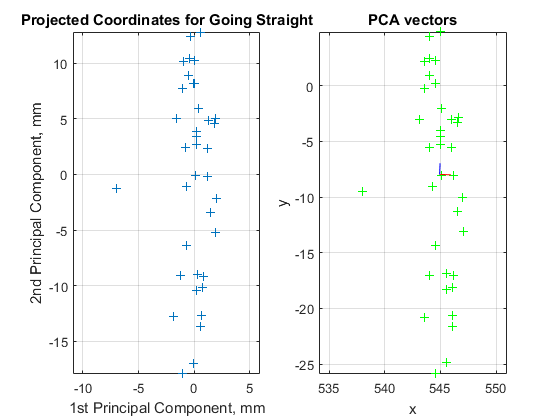
\includegraphics[scale=0.8]{s1}
\end{center}



\subsubsection{Slight left movement}

\begin{center}
  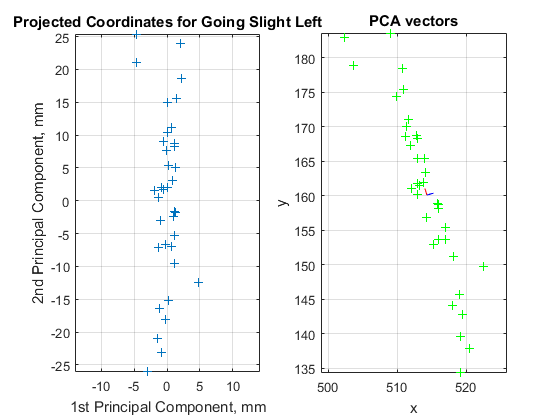
\includegraphics[scale=0.8]{l1}
\end{center}


\subsubsection{Slight right movement}

\begin{center}
  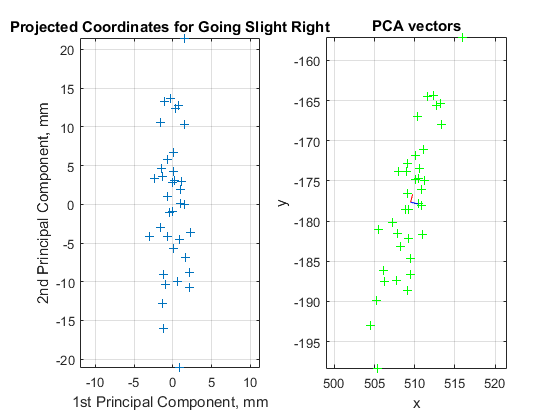
\includegraphics[scale=0.8]{r1}
\end{center}


\subsubsection{Left movement}

\begin{center}
  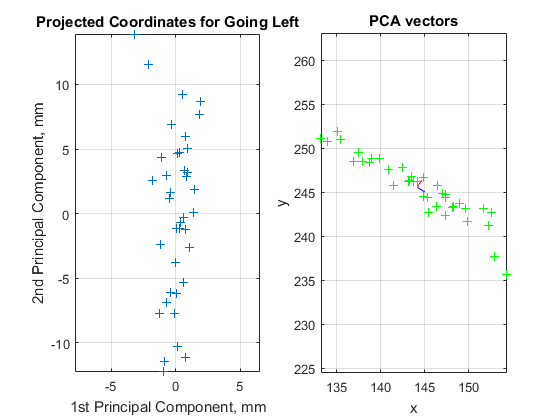
\includegraphics[scale=0.8]{ll1}
\end{center}


\subsubsection{Right movement}

\begin{center}
  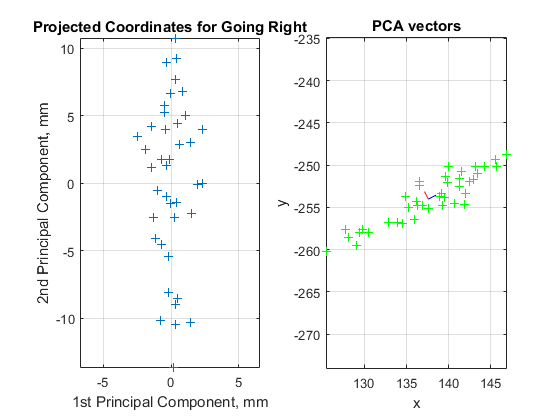
\includegraphics[scale=0.8]{rr1}
\end{center}

\newpage

Matlab code of PCA function:

\lstinputlisting{fitGaussian.m}



\section{Chi square test}
After projecting the data on principal coordinate vectors, chi square test can be performed. In my implementation, confidence level can be chosen. Test checks if data fits Gaussian distribution with $\mu = \mu_{empirical}$ and $\sigma = \sigma_{empirical}$.

The following figures shows histograms of data projections on principal vectors and angular deviation from mean value. Additionally it shows results of a Pearson chi-square test.

\newpage

\subsubsection{Straight movement}

\begin{center}
  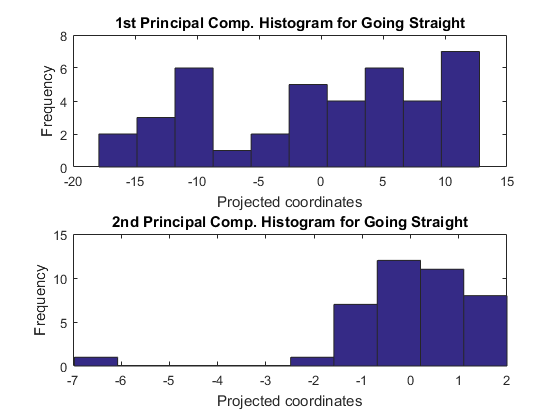
\includegraphics[scale=0.6]{s2}
  
  
  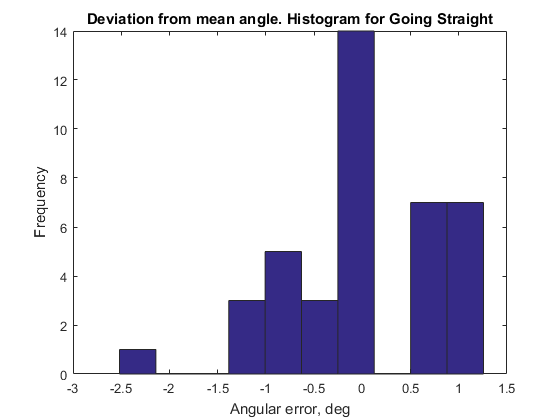
\includegraphics[scale=0.6]{s3}
\end{center}

Data: projection of 1st principal component during  Straight movement, is Gaussian distributed with: mean = 0 and standard deviation sigma = 8.9302 with confidence 0.9%.


\smallskip

Data:  projection of 2st principal component during  Straight movement, can not be proven to have Gaussian Distribution with confidence 0.9%.


\smallskip


Data: angular error during   Straight movement, is Gaussian distributed with: mean = 0 and standard deviation sigma = 0.82481 with confidence 0.9%.

\begin{table}[!h]
\centering
\caption{Experimental results: straight movement}
\begin{tabular}{lllll}
     & Desired & Mean value & Accuracy & Precision \\
x    &  558  mm     &    545  mm      &    13  mm    &     9  mm    \\
y    &  0  mm     &     -8  mm     &  8    mm    &    -       \\
$\phi$ &  0   deg    &     -2.3    deg   &     2.3 deg     & 0.8 deg
\end{tabular}
\end{table}


\newpage
\subsubsection{Slight left movement}

\begin{center}
  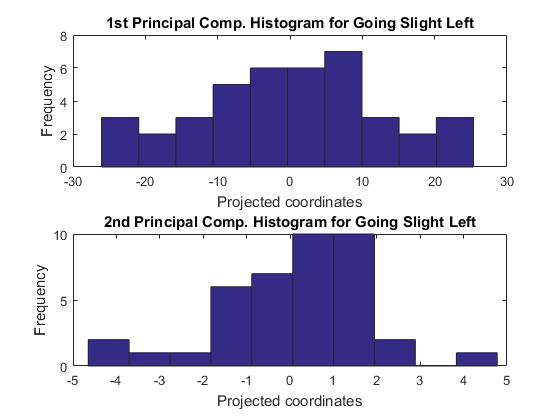
\includegraphics[scale=0.6]{l2}
  
  
  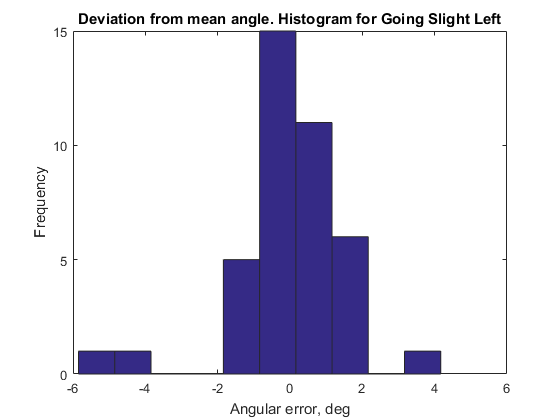
\includegraphics[scale=0.6]{l3}
\end{center}


Data: projection of 1st principal component during  Slight Left movement, is Gaussian distributed with: mean = 0 and standard deviation sigma = 12.7958 with confidence 0.9%.



\smallskip

Data: projection of 2st principal component during  Slight Left movement, is Gaussian distributed with: mean = 0 and standard deviation sigma = 1.7139 with confidence 0.9%.



\smallskip


Data:  angular error during   Slight Left movement, can not be proven to have Gaussian Distribution with confidence 0.9%.

\begin{table}[!h]
\centering
\caption{Experimental results: slight left movement}
\begin{tabular}{lllll}
     & Desired & Mean value & Accuracy & Precision \\
x    &  530  mm     &    514  mm      &    16  mm    &     13  mm    \\
y    &  160 mm     &     160  mm     &  0    mm    &    2   mm    \\
$\phi$ &  30   deg    &     30    deg   &     0 deg     & - deg
\end{tabular}
\end{table}

\newpage
\subsubsection{Slight right movement}

\begin{center}

  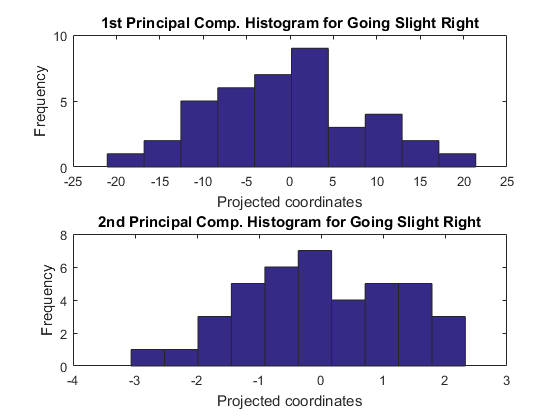
\includegraphics[scale=0.6]{r2}
  
  
  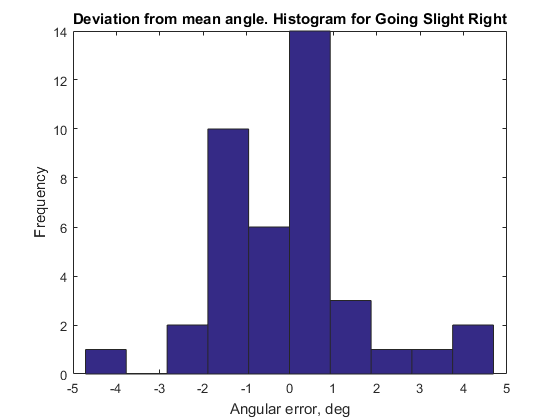
\includegraphics[scale=0.6]{r3}
\end{center}


Data: projection of 1st principal component during  Slight Right movement, is Gaussian distributed with: mean = 0 and standard deviation sigma = 8.8624 with confidence 0.9%.




\smallskip

Data: projection of 2st principal component during  Slight Right movement, is Gaussian distributed with: mean = 0 and standard deviation sigma = 1.2828 with confidence 0.9%.




\smallskip


Data: angular error during   Slight Right movement, is Gaussian distributed with: mean = 0 and standard deviation sigma = 1.7816 with confidence 0.9%.

\begin{table}[!h]
\centering
\caption{Experimental results: slight right movement}
\begin{tabular}{lllll}
     & Desired & Mean value & Accuracy & Precision \\
x    &  530  mm     &    509  mm      &    21  mm    &     9  mm    \\
y    &  -160 mm     &     -177  mm     &  17    mm    &    1 mm      \\
$\phi$ &  -30   deg    &     -34    deg   &     4 deg     & 2 deg
\end{tabular}
\end{table}

\newpage
\subsubsection{Left movement}

\begin{center}
  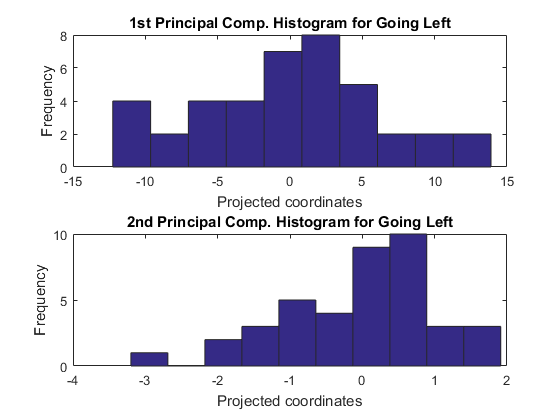
\includegraphics[scale=0.6]{ll2}
  
  
  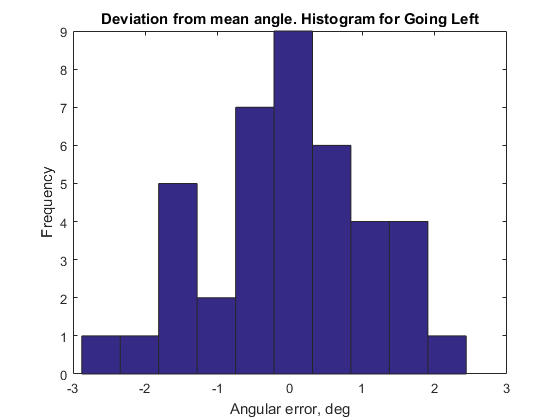
\includegraphics[scale=0.6]{ll3}
\end{center}


Data: projection of 1st principal component during  Left movement, is Gaussian distributed with: mean = 0 and standard deviation sigma = 6.382 with confidence 0.9%.





\smallskip

Data: projection of 2st principal component during  Left movement, is Gaussian distributed with: mean = 0 and standard deviation sigma = 1.0773 with confidence 0.9%.





\smallskip


Data: angular error during   Left movement, is Gaussian distributed with: mean = 0 and standard deviation sigma = 1.2094 with confidence 0.9%.

\begin{table}[!h]
\centering
\caption{Experimental results: left movement}
\begin{tabular}{lllll}
     & Desired & Mean value & Accuracy & Precision \\
x    &  180  mm     &    144  mm      &    36  mm    &     6  mm    \\
y    &  250 mm     &    245  mm     &  5    mm    &    1   mm    \\
$\phi$ &  90   deg    &     85    deg   &     5 deg     & 1 deg
\end{tabular}
\end{table}

\newpage
\subsubsection{Right movement}

\begin{center}
  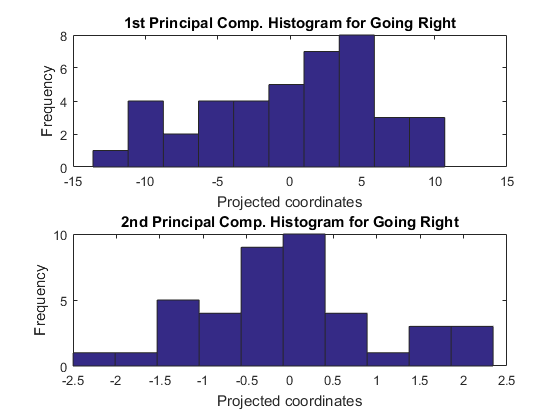
\includegraphics[scale=0.6]{rr2}
  
  
  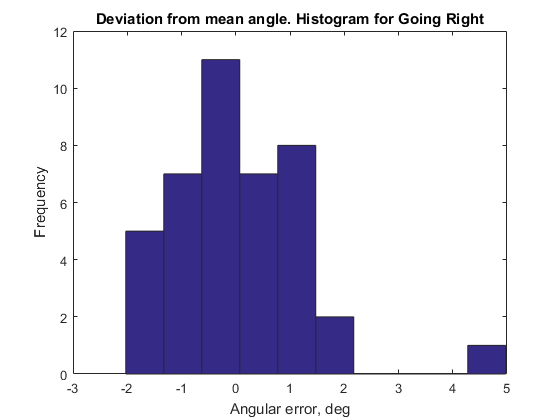
\includegraphics[scale=0.6]{rr3}
\end{center}


Data: projection of 1st principal component during  Right movement, is Gaussian distributed with: mean = 0 and standard deviation sigma = 6.0358 with confidence 0.9%.






\smallskip

Data: projection of 2st principal component during  Right movement, is Gaussian distributed with: mean = 0 and standard deviation sigma = 1.0768 with confidence 0.9%.






\smallskip


Data:  angular error during   Right movement, can not be proven to have Gaussian Distribution with confidence 0.9%.

\begin{table}[!h]
\centering
\caption{Experimental results: right movement}
\begin{tabular}{lllll}
     & Desired & Mean value & Accuracy & Precision \\
x    &  180  mm     &    137  mm      &    43  mm    &     6  mm    \\
y    &  -250 mm     &    -254  mm     &  4    mm    &    1   mm    \\
$\phi$ &  -90   deg    &     -81    deg   &     9 deg     & - deg
\end{tabular}
\end{table}

\newpage

\subsubsection{Matlab code of chi square test function:}

\lstinputlisting{chiSquareTestGaussian.m}

\section{Results/ conclusion}

\begin{itemize}
\item Experimental results have better precision than accuracy.
\item The robot is biased to the right.
\item The robot has higher error in $x$ direction.
\item Data contain some outliers that spoil Gaussian hypothesis.
\item Some distributions seem to be not gaussian.
\end{itemize}




\end{document}
